\chapter{Compute architecture and scheduling}
\begin{center}
    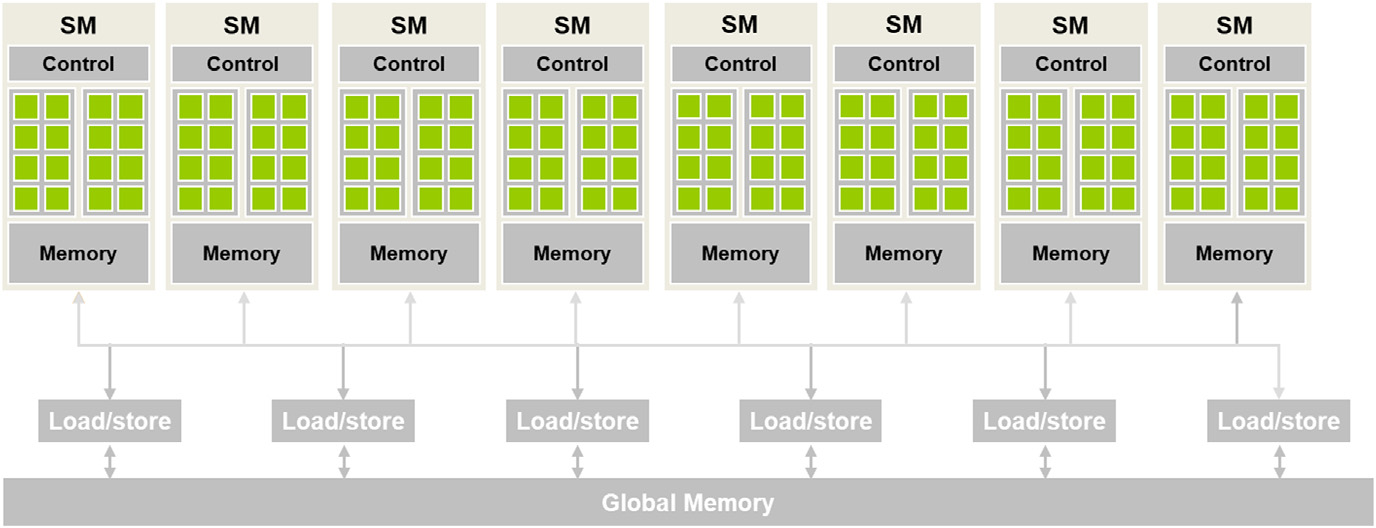
\includegraphics[width=0.7\linewidth]{Images/CompArch/CUDA_GPU.png}
\end{center}
\begin{itemize}
    \item A CUDA capable GPU is organized into an array of highly threaded streaming multiprocessors(SMs).
          \begin{itemize}
              \item Each SM $\rightarrow$ has several processing units called CUDA Cores (cores).
                    \begin{itemize}
                        \item Each Core $\rightarrow$ shares control logic and memory resources.
                    \end{itemize}
          \end{itemize}
\end{itemize}

\section{Block scheduling}
\begin{center}
    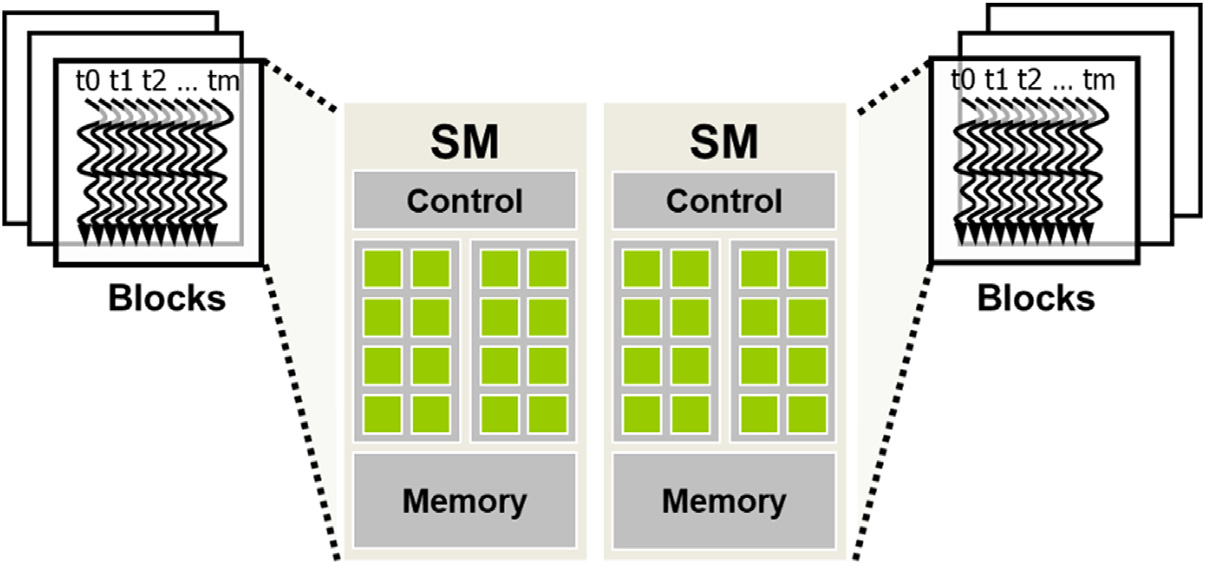
\includegraphics[width=0.7\linewidth]{Images/CompArch/block_assignment.png}
\end{center}
When the kernel is called, the CUDA runtime system launches a grid of threads that execute kernel code. The threads are attached to Streaming Multiprocessors (SMs) on a block-by-block basis.
\begin{itemize}
    \item i.e, \textbf{all the threads in a block are assigned to the same SM}.
    \item Multiple blocks are assigned to the same SM.
    \item \textbf{Blocks need to reserve hardware resources} to execute. $\implies$ A \textbf{limited number of blocks can be assigned to an SM.}
          \begin{itemize}
              \item As the \textbf{number of SMs} in a GPU is \textbf{limited}, the \textbf{total number of blocks that can be simultaneously executing on a CUDA device is limited}.
              \item Most grids contain many more blocks than this number. To ensure all the blocks in a grid get executed, the runtime system maintains a list of blocks that need to execute and assigns new blocks to SMs when previously assigned blocks complete execution.
          \end{itemize}
    \item This fashion of assignment of threads to SMs \textbf{guarantees that the threads in the same block are scheduled simultaneously on the same SM}. This \textbf{guarantee enables the threads in the same block to interact with each other} in ways that the threads across the blocks cannot.
\end{itemize}

\section{Synchronization and transparent scalability}
\subsection{\_\_syncthreads()}
\begin{itemize}
    \item The threads from the same block can coordinate their activities using the barrier synchronization function \texttt{\_\_syncthreads()}.
    \item If a thread calls \texttt{\_\_syncthreads()}, the thread will be held at the program location of the call, until all threads in the block reach that location. Ensures all the threads have completed a phase of their execution before moving to the next phase.
          \begin{center}
              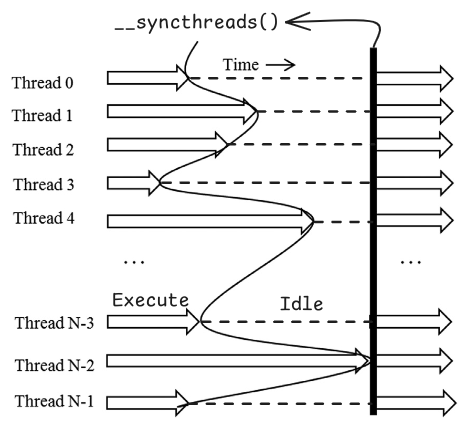
\includegraphics[width=0.7\linewidth]{Images/CompArch/syncthreads.png}
          \end{center}
    \item Among the \textsl{N threads} in the image above, the $\textsl{N-2 }^{nd}$ thread is the last to execute. But all the other threads wait for the $\textsl{N-2 }^{nd}$ thread to finish the execution, thus ensuring the same program location / state among all the threads in the block.
    \item With barrier synchronization, \enquote{no one is left behind.}
    \item In CUDA, if a \textbf{\texttt{\_\_syncthreads()}} statement is present, it \textbf{must be executed by all threads in a block}.
    \item \textbf{\texttt{\_\_syncthreads()}} in \texttt{if} block: The \texttt{\_\_syncthreads()} is \textbf{either executed by all the threads or none of the threads} in the block.
    \item \textbf{\texttt{\_\_syncthreads()}} in \texttt{if-else} block: if each path has \texttt{\_\_syncthreads()} statement, then either all the threads execute the \texttt{if-then} path or \texttt{else} path. The two \item \textbf{\texttt{\_\_syncthreads()}} in \texttt{if block} are different barrier synchronization points. Since not all threads in a block are guaranteed to execute the same barrier, the code violates the rules for using \textbf{\texttt{\_\_syncthreads()}} and will result in undefined execution behavior.
          \begin{minted}{cpp}
        void incorrect_barrier_example(int n){
            ...
            if (threadIdx.x % 2 == 0) {
                ...
                // All the even threads wait here. 
                __syncthreads();
            }
            else {
                ...
                // All the odd threads wait here. 
                __syncthreads();
            }
        }
    \end{minted}
    \item Barrier synchronization \textbf{imposes execution constrains on the threads within a block}. \textbf{The threads should operate in close time proximity with each other to avoid excessively long waiting times.}
    \item The \textbf{system needs to make sure that all the threads involved in synchronization should have the access to necessary resources to arrive at the barrier}. Otherwise, a thread may never arrive at barrier synchronization point, which \textbf{can cause a deadlock}.\\
          \linebreak
          $\implies$ All threads of the block should be assigned to the same SM, but should be assigned simultaneously to the SM (whole block executes once). i.e, a block can begin execution only when the runtime system has secured all the resources needed by all threads in the block to complete execution. Ensuring the time proximity of all threads in a block preventing excessive or indefinite waiting time during barrier synchronization.

\end{itemize}
\subsection{Transparent scalability}
\begin{itemize}

    \item As the threads from different blocks can't communicate with one another, CUDA runtime system can execute the blocks in any order relative to each other. This flexibility enables scalable implementations.
          \begin{center}
              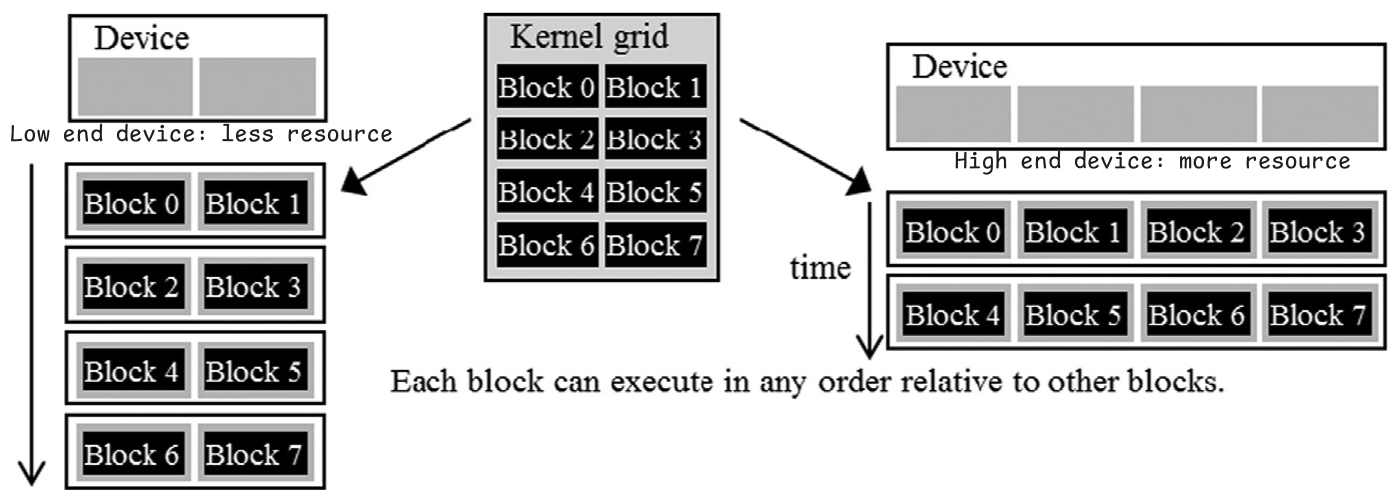
\includegraphics[width=0.9\linewidth]{Images/CompArch/Scaling.png}
          \end{center}
    \item The ability to execute the same application code with a wide range of speeds allows the production of a wide range of implementations according to the cost, power, and performance requirements of different market segments.
    \item The ability to execute the same application code on different hardware with different amounts of execution resources is referred to as \textbf{\textit{transparent scalability}}, which reduces the burden on application developers and improves the usability of applications.

\end{itemize}

\section{Warps and SIMD hardware}
\begin{itemize}
    \item One should assume that in a block, threads can execute in any order w.r.t to each other.
    \item In algorithms with phases, barrier synchronization should be used between all the threads in a block, whenever the threads must move from one phase to the other. The \textbf{correctness of executing a kernel} \textbf{\textit{shouldn't}} \textbf{depend on any assumption that threads will synchronize without the use of barrier synchronization}.
\end{itemize}

\subsection{Warps}
\begin{itemize}
    \item A block is further divided into 32-thread units called warps. \textit{The size of the warps can vary in the future.} A warp is the unit of thread scheduling in SMs.
          \begin{center}
              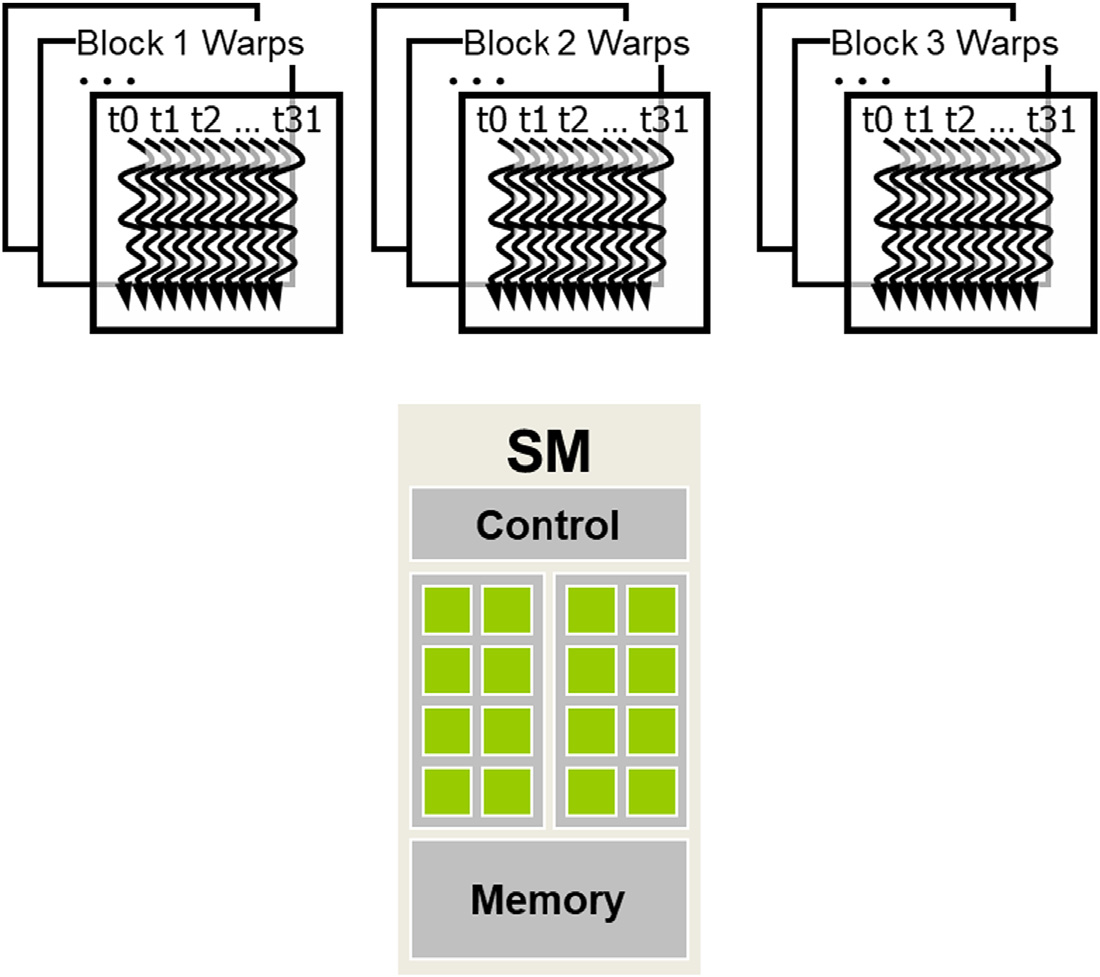
\includegraphics[width=0.8\linewidth]{Images/CompArch/Warps.png}
          \end{center}
    \item Block 1, Block 2, Block 3 - all are assigned to the single SM. Each block is further divided into warps for scheduling purposes.
          \begin{itemize}
              \item Each warp consists of 32 consecutive \texttt{threadIdx} values: threads 0 through 31 form the first warp, threads 32 through 64 the second warp etc.
              \item If each block has 256 threads, a block has 256/32 = 8 warps.
              \item With 3 blocks in the SM, there are 8 $\times$ 3 = 24 warps in the SM.
          \end{itemize}
    \item Block $\rightarrow$ Warp: Index $z$ axis, then $y$ then $x$.
          \begin{center}
              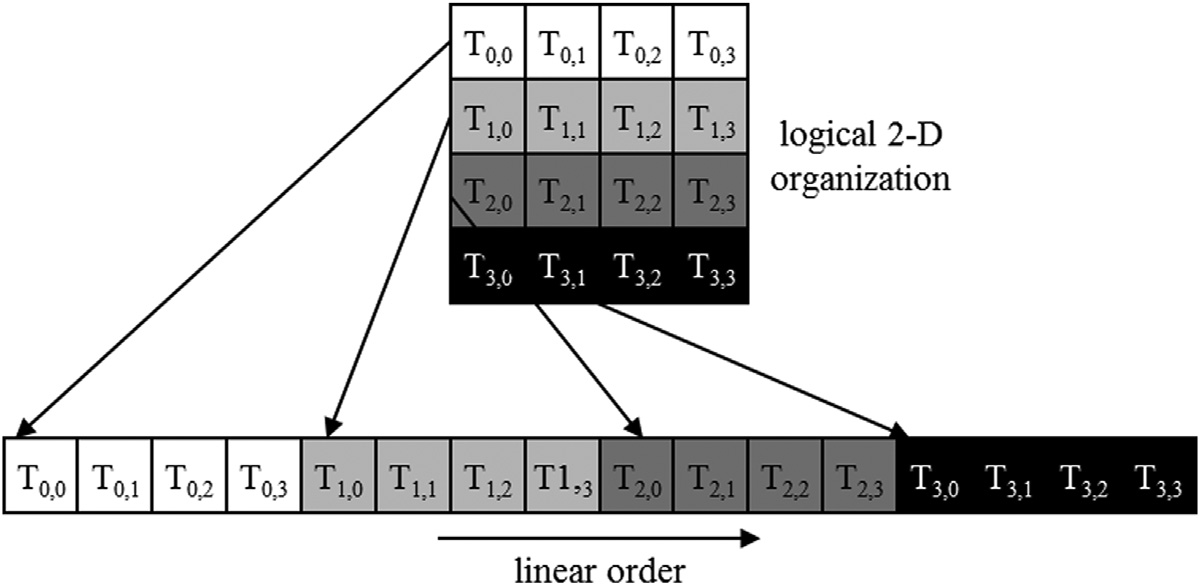
\includegraphics[width=0.7\linewidth]{Images/CompArch/Unrwrapping.png}
          \end{center}
    \item For 2D grid: $T_{\text{y,x}}$, y being \texttt{threadIdx.y} and x being \texttt{threadIdx.x}, a 2D grid is linearized by placing all the threads whose \texttt{threadIdx.y} is 0 then \texttt{threadIdx.y} is 1 and so on. Threads with the same threadIdx.y value are placed in consecutive positions in increasing threadIdx.x order.
    \item In the above figure, the 16 threads form half a warp. The warp is padded with 16 other threads to form a 32-thread warp.
    \item 2D Block with 8 $\times$ 8 threads form 2 warps of 32 threads.\\ Warp 1: $\text{T}_{0,0}$ to $\text{T}_{3,7}$\\ warp 2: $\text{T}_{4,0}$ to $\text{T}_{7,7}$
    \item 3D Block with 2 $\times$ 8 $\times$ 4 threads, form 2 warps of 32 threads. \\warp 1: $\text{T}_{0, 0, 0}$ to $\text{T}_{0,7,3}$ \\ warp 2: $\text{T}_{1,0,0}$ to $\text{T}_{1, 7, 3}$
\end{itemize}

\subsection{SIMD}
\begin{center}
    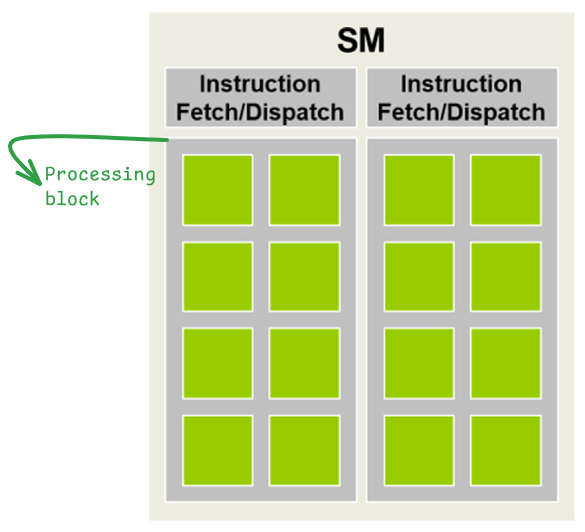
\includegraphics[width=0.3\linewidth]{Images/CompArch/SIMD_organization.png}
\end{center}
\begin{itemize}
    \item An SM is designed to execute all threads in a warp following the single-instruction, multiple-data (SIMD) model. That is, at any instant in time, one instruction is fetched and executed for all threads in the warp.
    \item As an example, in a GPU of 16 cores/SM, all the cores in a processing block share an instruction fetch/dispatch unit. \textbf{Threads in the same warp are assigned to the same processing block, which fetches the instruction for the warp and executes it for all the threads in the warp at the same time. These threads apply the same instruction to different portions of the data. Because the SIMD hardware effectively restricts all threads in a warp to execute the same instruction at any point in time, the execution behavior of a warp is often referred to as single instruction, multiple-thread.}
    \item The \textbf{advantage of SIMD} is that the \textbf{cost of the control hardware}, such as the instruction fetch/dispatch unit, \textbf{is shared across many execution units}. This design choice \textbf{allows for a smaller percentage of the hardware to be dedicated to control and a larger percentage to be dedicated to increasing arithmetic throughput}.
\end{itemize}

\subsubsection{- von Neuman Model}
\begin{center}
    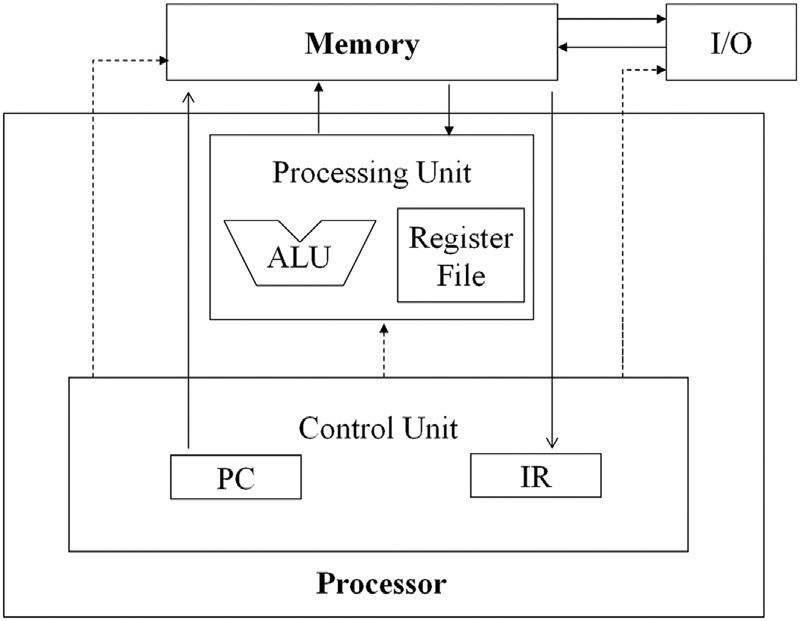
\includegraphics[width=0.4\linewidth]{Images/CompArch/neuman.png}
\end{center}
\begin{itemize}
    \item The computer has an I/O (input/output) that allows both programs and data to be provided to and generated from the system.
    \item Computer loads the program and data into memory, before executing the program. Program is a set of instructions.
    \item The \textsl{Control Unit} maintains a \textsl{Program Counter}(PC), which contains the memory address of the next instruction that is to be executed.
    \item In each \textsl{\enquote{instruction cycle}}, the \textsl{Control Unit} uses the \textsl{PC} to fetch an instruction into the \textsl{Instruction Register}(IR).
    \item The instruction bits are then examined to determine the action to be taken by all the components of the computer.
\end{itemize}

\subsubsection{- Modified von Neuman Model for SIMD}
\begin{center}
    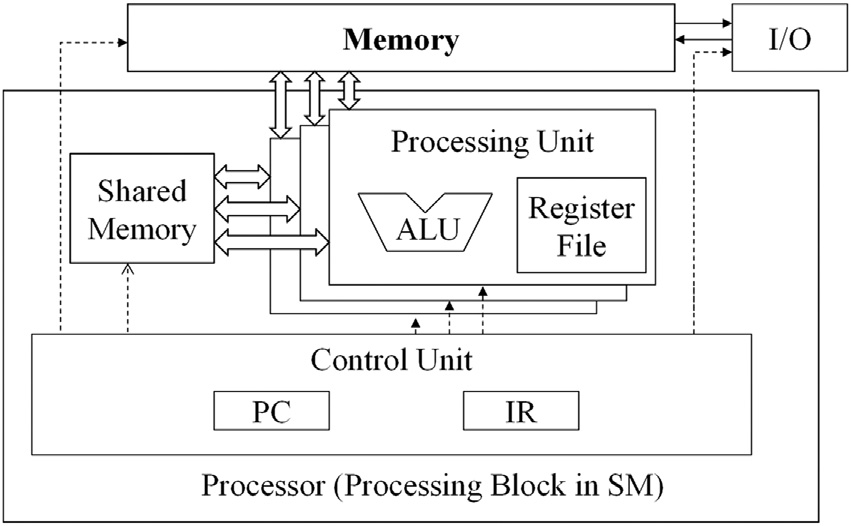
\includegraphics[width=0.5\linewidth]{Images/CompArch/neuman_simd.png}
\end{center}
\begin{itemize}
    \item Since all processing units are controlled by the same \textsl{Instruction Register} (IR) of the \textsl{Control Unit}, the only execution differences in these units are the input data (in register files) on which they operate on.
    \item This is \textsl{Single Instruction Multiple-Data} in processor design.
    \item Control units in modern processors are complex and sophisticated for fetching instructions and access instruction cache. Having multiple processing units share the same control unit can result in significant reduction in hardware manufacturing and power consumption.
\end{itemize}

\section{Control Divergence}
\textbf{SIMD provides massive performance gains when all the threads within a warp follow the same execution path, or \textit{control flow}} when working on their data.\\
For example, in an \texttt{if-else} construct, the execution works well when either all the threads follow the \texttt{if}-path or all execute the \texttt{else}-path.\\
However, when the threads in the warp take different control paths, the SIMD hardware has to take multiple passes through these paths, with one pass per each path.
\begin{itemize}
    \item When threads in the same warp follow different execution paths, we say that these threads exhibit control divergence, that is, they diverge in their execution.
    \item While the \textbf{hardware} executes the same instruction for all threads in a warp, it \textbf{selectively lets these threads take effect in only the pass that corresponds to the path that they took}, allowing every thread to appear to take its own control flow path.
    \item This preserves the independence of threads while taking advantage of the reduced cost of SIMD hardware.
    \item The cost of divergence, however, is the extra passes the hardware needs to take as well as the execution resources the inactive threads consume in each pass.
\end{itemize}
\subsubsection{- Example: \texttt{if-else-loop}}
\begin{center}
    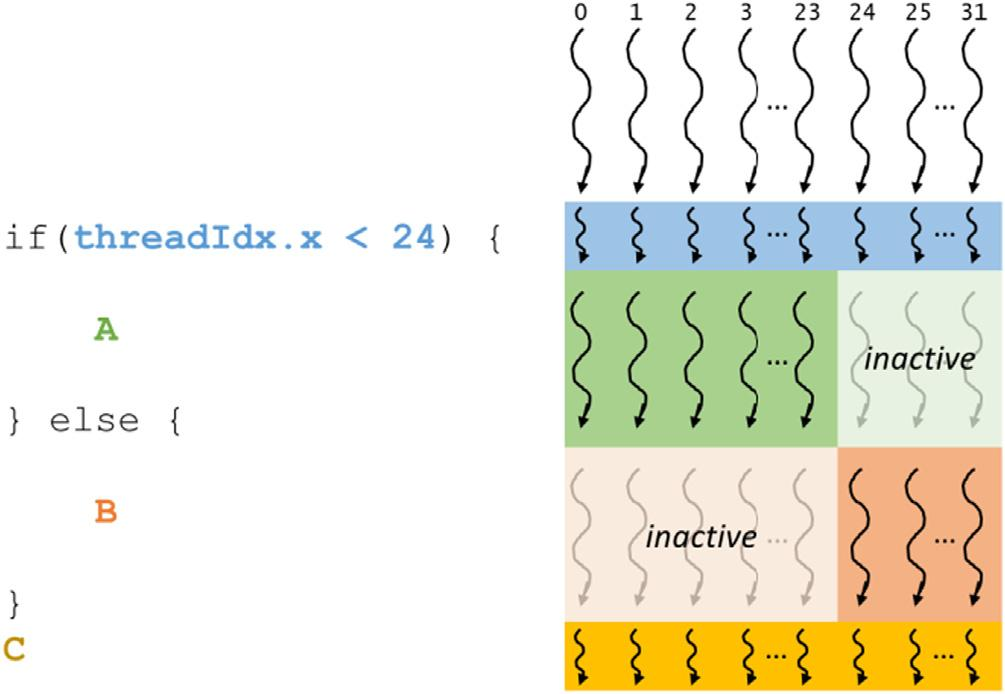
\includegraphics[width=0.6\linewidth]{Images/CompArch/control_divergence_ifelse.png}
\end{center}
\begin{itemize}

    \item First Pass:
          \subitem threads with $\texttt{threadIdx.x} < 24$ execute \texttt{A}.
          \subitem threads with  $24 < \texttt{threadIdx.x} <= 32$ are inactive.
    \item Second Pass:
          \subitem threads with  $24 < \texttt{threadIdx.x} <= 32$ execute \texttt{B}.
          \subitem threads with $\texttt{threadIdx.x} < 24$ are inactive.
    \item The threads in the warp reconverge and then execute \texttt{C}.
    \item From the Volta architecture onwards, the passes may be executed concurrently, meaning that the execution of one pass may be interleaved with the execution of another pass, known as \textit{independent thread scheduling}.
\end{itemize}

\subsubsection{- Example: \texttt{for-loop}}
\begin{center}
    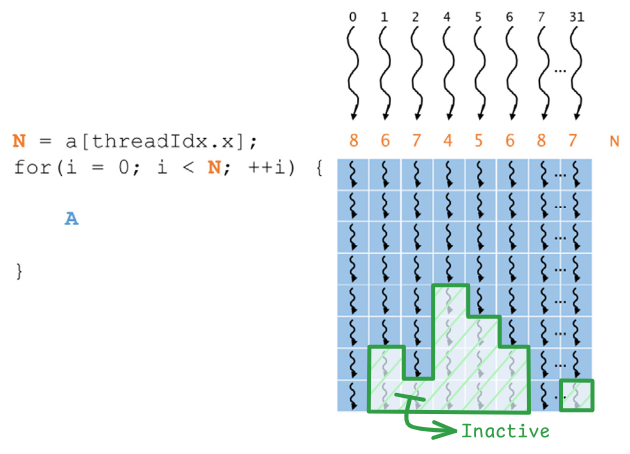
\includegraphics[width=0.5\linewidth]{Images/CompArch/control_divergence_for.png}
\end{center}

\begin{itemize}
    \item The for loop varies between 4 and 8.
    \item For the first four iterations, all threads are active and execute A.
    \item For the remaining iterations, some threads execute A, while others are inactive because they have completed their iterations.
\end{itemize}

\subsubsection{- To guess thread/control divergence}
\begin{itemize}
    \item If the decision condition is based on threadIdx values, the control statement can potentially cause thread divergence.
    \item For example, the statement \texttt{if(threadIdx.x $>$ 2) \{\dots\}} causes the threads in the first warp of a block to follow two divergent control flow paths.
          \subitem Threads 0, 1, and 2 follow a different path than that of threads 3, 4, 5, and so on.
\end{itemize}

\subsubsection{- Reasons to use control construct with thread control divergence}
\begin{itemize}
    \item To handle boundary conditions when mapping threads to data.
          \begin{itemize}

              \item \textbf{Example}: Vector length: 1003, Block size: 64 $\implies$ (1003 + 64 - 1)/64, i.e, 16 thread blocks to process the 1003 elements.
              \item 16 thread blocks $\rightarrow$ have 1024 total threads.
              \item We need to disable the last 21 threads in thread block 15 from doing work that is not expected or not allowed by the original program.
              \item The 16 blocks are partitioned into 32 warps. \textbf{Only the last warp} (i.e., the second warp in the last block) \textbf{will have control divergence.}
          \end{itemize}
    \item The performance impact of control divergence decreases as the size of the vectors being processed increases.
          \begin{itemize}
              \item For a vector length of 100, one of the four warps will have control divergence. (25\%)
              \item For a vector size of 1000, only one of the 32 warps will have control divergence. (4\%)
              \item For a vector of length 10,000, only one of the 313 warps will have control divergence. (0.3\%)
          \end{itemize}
    \item Due to the control divergence, one can not confidently assume that all the threads in the warp have the same execution timing. If all threads in a warp must complete one phase before moving to the next phase, barrier synchronization mechanism such as \texttt{\_\_syncwarp()} is to be used.
\end{itemize}
